Mediante datos satelitales y en algunos casos mediante observación directa, se han detectado en Julio de 2021,  incendios en las islas del río Paraná, en la zona que está comprendida entre San Nicolás y San Lorenzo.\\

Los focos de incendios se contabilizaron con un programa propio en el área del humedal (Figura \ref{fig:satelital}). Los datos provienen del instrumento satelital VIIRS-Suomi NOAA-20, especializado en la detección de focos de incendio que forma parte de la Plataforma FIRMS/NASA.

\begin{figure}[H]
    \centering
    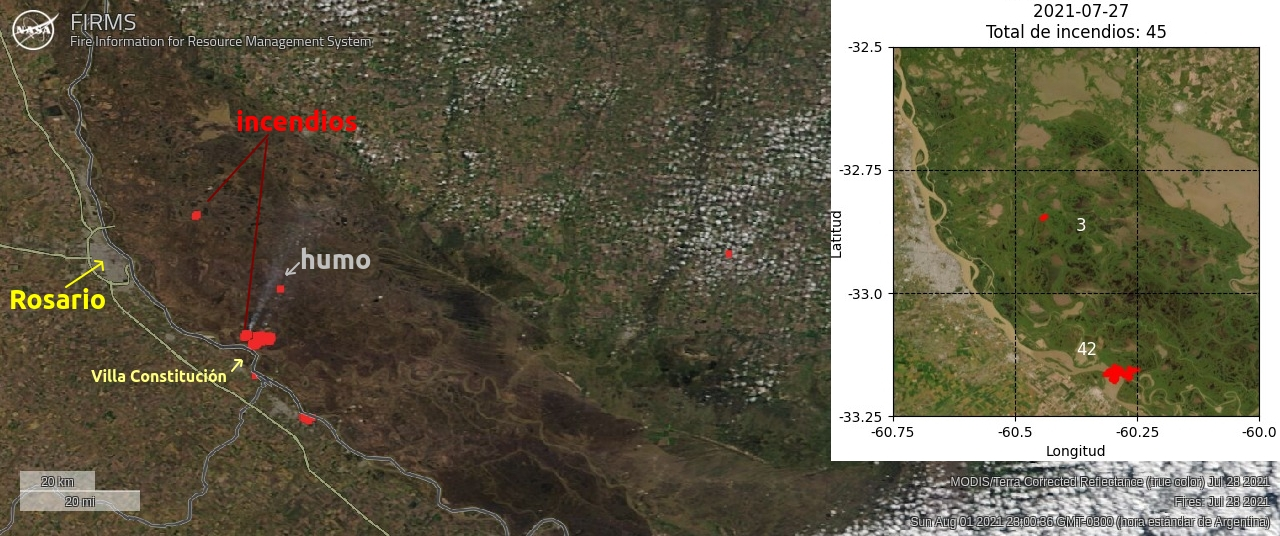
\includegraphics[width=0.75\paperwidth]{images/image3.jpg}
    \caption{Imagen satelital de la plataforma FIRMS/NASA, editada con la ubicación de Rosario y Villa Constitución el día 28/Julio/2021. En el recuadro derecho se muestra una imagen del programa contabilizador de focos de incendio para el día 27/Julio/2021.}
    \label{fig:satelital}
\end{figure}


En la Figura \ref{fig:satelital} se muestran el número y ubicación de focos de incendios, excluyendo los puntos sobre las ciudades de Villa Constitución y San Nicolás, que con frecuencia son señalados como focos incendios debido a la alta temperatura generada por la actividad industrial. Los días 27 y 28 de Julio fueron detectados incendios frente a Rosario, ambos días el viento fue en dirección SSO.\\

En particular, entre el viernes 30 de Julio y el domingo 1 de Agosto 2021 (Figura \ref{fig:quema_de_biomasa}), se detectaron eventos de humo en Rosario y región. Muy posiblemente estos eventos están ligados a incendios que se registraron en las islas del Paraná debido a que el 1 de Agosto, los vientos fueron a lo largo del día en las direcciones: SSE, SSO y S. El Servicio Meteorológico Nacional registró la presencia de humo al comienzo de la mañana y el olor a humo fue sentido por personas sensibles, aún en la vecina ciudad de Funes.\\

Se observó la presencia de restos de vegetal quemado en el suelo de la zona de La Florida, de dimensiones que van desde algunos milímetros a varios centímetros, siendo su concentración superficial diaria de unos 0.5 trozos quemados por cada metro cuadrado (Figura \ref{fig:quema_de_biomasa}). Tanto el humo (conteniendo gases y material particulado microscópico) como estos trozos de biomasa quemada, son factores que afectan, no sólo los objetos y construcciones al exterior sino también la salud humana, ya que estos últimos con el paso del tiempo se destruyen, transformándose en gran medida en aerosoles.\\

\begin{figure}[H]
    \centering
    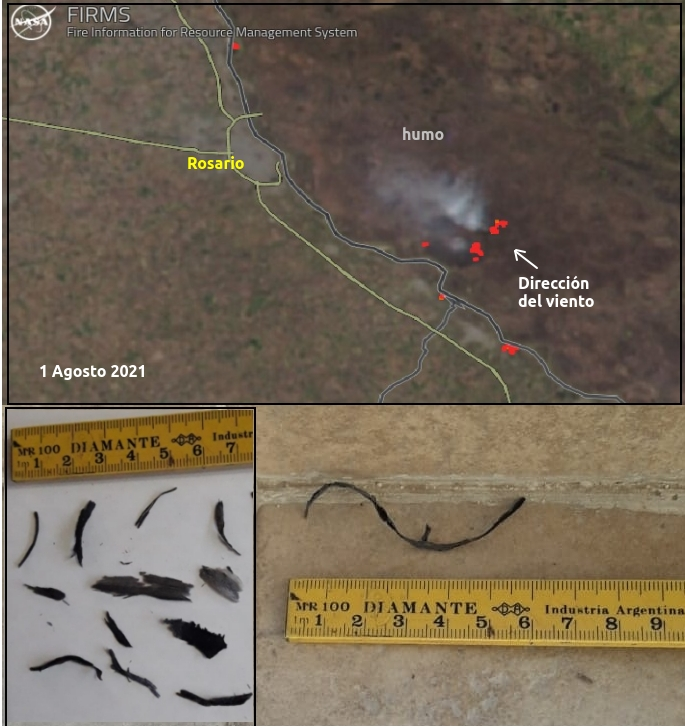
\includegraphics[width=0.6\paperwidth]{images/image2.jpg}
    \caption{Arriba. Imagen satelital obtenida el 1 de Agosto 2021 por FIRMS/NASA. Izquierda. Trozos de quema de biomasa de las islas recogidos en barrio La Florida, Rosario que se depositaron del 30 de Julio al 1 de Agosto 2021, con una densidad superficial de alrededor de 0.5 trozo/(m\textsuperscript{2}.día). Derecha. Fotografía del mayor resto  depositado en piso en el mismo periodo y lugar geográfico.}
    \label{fig:quema_de_biomasa}
\end{figure}

El Sistema de Alerta Temprana (SAT) reportó el PM2.5 máximo diario que superó los 100 $\mu$gr/m\textsuperscript{3} durante el mes de Julio 2021, así como los días de precipitación acumulada. El número de incendios en esta zona registrados en los distintos días del mes de Julio, muestran una relación directa en el día del valor máximo mensual con el incremento del número de partículas microscópicas en la atmósfera, denominadas aerosoles (Figura \ref{fig:incendios}).

\begin{figure}[H]
    \centering
    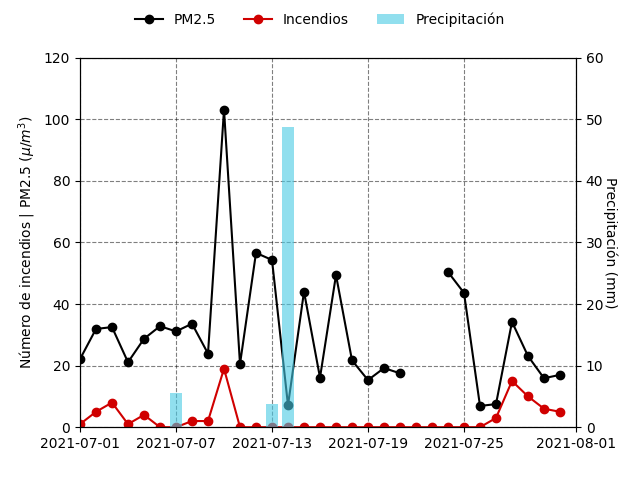
\includegraphics[width=0.4\paperwidth]{images/image1.png}
    \caption{Número de focos de incendios detectados por el equipo satelital VIIRS-Suomi-NOAA-20 y material particulado PM\textsubscript{2.5} y precipitación, registrados por el Sistema de Alerta Temprana (SAT).}
    \label{fig:incendios}
\end{figure}

Mediante el análisis de datos satelitales aportados por los organismos oficiales NOAA y NASA de Estados Unidos, se contabilizó el número de incendios durante el mes de Julio 2021. Al menos dos días de ese mes, este número mostró una relación directa con la máxima concentración diaria de material particulado en la atmósfera, medida por el Sistema de Alerta Temprana de Granadero Baigorria. Otra confirmación de la fuente de este material particulado fue dada por imágenes satelitales, donde se observa que el viento del Sureste dirigió la nube de humo desde la zona de las islas frente a Villa Constitución, hacia Rosario y región cercana. También fue posible registrar restos de vegetación quemada en el suelo de la zona de La Florida, de dimensiones que van desde algunos milímetros a varios centímetros. Para un adecuado monitoreo de la Calidad del Aire es necesario contar con una red de medición conformada por un conjunto de estaciones de muestreo automático o semiautomático de contaminantes (de partículas y contaminantes gaseosos) a lo largo del día. Este monitoreo tiene la finalidad de conocer el grado de exposición que tienen los habitantes de una región, a través del análisis de datos, tendencias y origen de dichos contaminantes, para lograr su control, regulación y prevención de efectos dañinos. Es fundamental que se reglamente el máximo de concentración de material particulado PM\textsubscript{2.5}, como ya existe en diversos países, para proteger la salud humana.\\

Los autores agradecen a los responsables del Sistema de Alerta Temprana (SAT), Granadero Baigorria, por la contribución de los datos de material particulado y precipitación.\vspace{1cm}
\hrule \vspace{0.25cm}
\small
Dra. \textbf{Adriana Ipiña}, investigadora del Instituto de Física Rosario, CONICET-UNR\\

\textbf{Gamaliel López-Padilla}, estudiante de la Facultad de Ciencias Físico-Matemáticas, UANL (México)\\

\textbf{Adelina Navarro}, estudiante de la Facultad de Ciencias Exactas Ingeniería y Agrimensura, UNR\\

\textbf{Dr. Rubén Piacentini}, investigador del Instituto de Física Rosario, CONICET-UNR
